\section{Smart Home}
\label{sec:smartHome}
    \acl{SH}, im Deutschen \textit{“intelligentes Zuhause“}, ist ein wesentliches Anwendungsgebiet des \acs{IoT}. 
    Diese Rubrik der Anwendung widmet sich überwiegend dem Gebrauch im privaten Umfeld und sämtlichen Haushaltsgeräten 
    und -einrichtungen. Ein kleiner Ausschnitt solcher Nutzgegenstände sind unter anderem Lampen, Kontaktsensoren, 
    Thermostate, Service-Roboter, Staubsauger-Roboter, Kühlschränke Geräte rundum die Haussicherheit. 
    \\ 
    Unter dem Oberbegriff \acl{SH} ist eine Weise zu verstehen, mit der die Erhöhung der Wohn- und Lebensqualität, 
    Energienutzung unter Verwendung vernetzter und fernsteuerbarer Geräten effizienter gestaltet, Sicherheit gesteigert 
    und Abläufe verschiedener Prozessschritte automatisiert werden kann.
    \\ 
    Der Begriff \textit{intelligentes Zuhause} wird verwendet, wenn die Haustechnik und Haushaltsgeräte untereinander 
    vernetzt sind. Die Definition im Deutschen Gebrauch, welche nach (Strese et al. 2010) in der Untersuchung im Rahmen 
    der wissenschaftlichen Begleitung zum Programm Next Generation Media (NGM) des Bundesministeriums für Wirtschaft und 
    Technologie aufgegriffen wird, lautet wie folgt: 
    \begin{quote}
        „Das Smart Home ist ein privat genutztes Heim (z.B. Eigenheim, Mietwohnung), in dem die zahlreichen Geräte der 
        Hausautomation (wie Heizung, Beleuchtung, Belüftung), Haushaltstechnik (wie z.B. Kühlschrank, Waschmaschine), 
        Konsumelektronik und Kommunikationseinrichtungen zu intelligenten Gegenständen werden, die sich an den 
        Bedürfnissen der Bewohner orientieren. Durch Vernetzung dieser Gegenstände untereinander können neue 
        Assistenzfunktionen und Dienste zum Nutzen des Bewohners bereitgestellt werden und einen Mehrwert 
        generieren, der über den einzelnen Nutzen der im Haus vorhandenen Anwendungen hinausgeht.“ \cite{strese.2010m}
    \end{quote}
    Eine vergleichbare Definition wurde zu späterem Zeitpunkt durch eine Literaturrecherche publiziert. Diese beschreibt 
    die zugrundeliegende Thematik weniger aus Anwendersicht sonder widmet sich vielmehr dem System und der Konnektivität. 
    \begin{quote}
        „A smart home is a place with heterogeneous systems to many
        front devices with the support of embedded information and
        communication architectures[...]“ \cite{Balakrishnan2018}
    \end{quote}
    Den beiden Definitionen ist zu entnehmen, dass die Kernaussage eine ähnliche ist, es jedoch in Büchern, Fachartikeln, 
    Publikationen an Universitäten und in den verbreiteten Medien bis heute keine durchgängige Definition gibt. Aus der
    % empirischen 
    einschlägigen Literatur wird ersichtlich, dass viele Synonyme für die Benennung der Thematik verwendet werden, darunter 
    beispielsweise: \cite{strese.2010m}
    \begin{itemize}
        \item Connected Home
        \item Elektronisches Haus
        \item Intelligentes Haus (engl. Smart House)
        \item Smart Living
        \item Home of the Future 
    \end{itemize}
    Eine elementare Information im Zusammenhang zu dieser Arbeit ist, dass die Verwendung des Begriffs \textit{intelligentes Büro} 
    ebenso in den Kontext des \acl{SH} gehört. Hierbei wird lediglich die Räumlichkeit im unternehmerischen Jargon verwendet, 
    die ebenso eine Grundlage für die Verwendung von Komponenten des \acl{SH} bietet. 
    \\
    An dieser Stelle wird deutlich, dass die Verwendung des Begriffs als auch die zugrundeliegenden technischen Verfahren 
    weiträumig einsetzbar sind und deshalb die Begriffsdefinition nicht eindeutig festgehalten werden kann. 
    
    \subsubsection*{Teilsysteme des \acl{SH}}
        Der Zentrale Punkt des \acl{SH} ist die Automatisierung häuslicher Prozesse. Dadurch sollen dem Nutzer 
        in vielerlei Hinsicht Aufwände erspart und Informationen zentralisiert angezeigt werden. Die Hausautomatisierung 
        umfasst eine Menge von Teilsystemen. Ein Ausschnitt dieser Teilsysteme ist der folgenden tabellarischen Auflistung zu entnehmen: 
        \begin{table}[hbt!]
            \begin{center}
                \begin{tabular}{| p{3cm} | p{12.75cm} | }
                    \hline
                        \textbf{Segment} & \textbf{Beschreibung} \\
                    \hline
                        Licht & Beleuchtung, Lichtmanagement/Szenarien, Storen/Rollos \\ 
                    \hline
                        Zutritt & Zutrittskontrolle, Klingelanlage, Schlösser, Anwesenheits- und Bewegungserfassung \\ 
                    \hline
                        Überwachung & Technische Alarme: Feuer, Rauch, Gas; Intrusion: Glasbruchmelder, Video; Babyphon, Urlaubswachschutz \\ 
                    \hline
                        Notfall & Sprinkleranlage, unabhängige Stromversorgung, Fluchtwegsystem \\ 
                    \hline
                        Metering & Verbrauchszähler für Strom, Gas, Wasser, Wärme, uvm. \\ 
                    \hline 
                        Konsumelektronik & TV, Internet, Smartphones, Tablets, Spielekonsolen etc. \\
                    \hline
                        Hausgeräte & Kühlschrank, Waschmaschine, Staubsauger, Service-Roboter; Hausgeräte-monitoring, -diagnostik, und -fernbedienung \\
                    \hline
                        Heimlogistik & Einkaufs- und Speiseplanung, häusliche Dienste \\ 
                    \hline
                        Hobby & Haustierversorgung, Aquarienmanagement, etc. \\
                    \hline
                        Mobilität & PKW mit Diagnostik, Navigationssystem mit local based services, Info-/Entertainmentangebote etc. \\ 
                    \hline
                \end{tabular}
            \end{center}
            \caption{Teilsysteme des Smart Home \cite{strese.2010m}}
            \label{tab:teilsysteme}
        \end{table}
        \\
        Ein weiterer wichtiger Anhaltspunkt zum Verständnis der Definition von Smart Home ist die Ausstattung der Komponenten mit Intelligenz und die 
        Vernetzung der Teilsysteme. Dadurch steht als Ziel im Vordergrund weniger die übergeordnete zentrale Steuerung, sondern vielmehr die verteilte 
        Intelligenz, um Aufgaben möglichst autonom (eigenständig) abzuarbeiten. Die dabei erzeugten als auch erforderlichen Daten mit anderen 
        Komponenten des Gesamtsystems auszutauschen, ist ebenso ein vorangestelltes Ziel, welches eine intelligente Umgebung schafft. 
        \\
        Eine mögliche Vernetzung und auch Verwendung solcher Komponenten wird in folgender Abbildung (\ref{pic:szenarien-smarhome}) 
        skizziert. Diese Grafik dient als grobe Übersicht potentieller Anwendungsszenarien, repräsentiert jedoch nicht alle Möglichkeiten der Anwendung. %ist allerdings nicht als vollständig zu interpretieren. 
        \begin{figure}[hbt!]
            \centering
            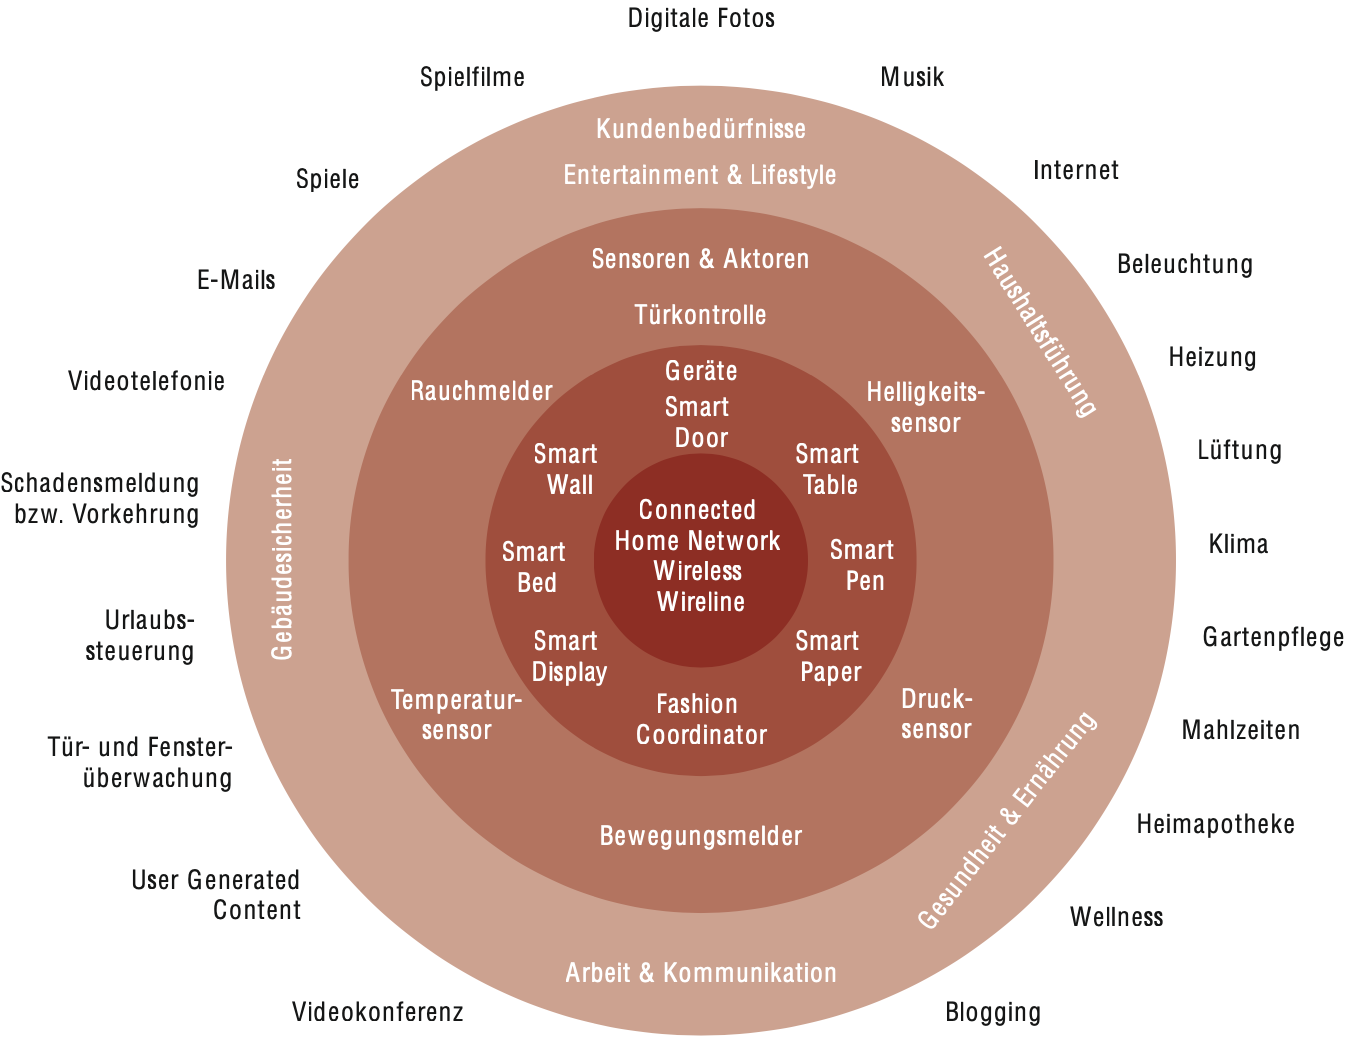
\includegraphics[width=15cm,height=15cm,keepaspectratio]{images/Anwendungsszenarien_SH.png}
            \caption{Mögliche Anwendungsszenarien im Smart Home \cite{strese.2010m}}
            \label{pic:szenarien-smarhome}
        \end{figure}
        \\
        Darüber hinaus gibt es weitaus mehrere Anwendungsszenarien, beziehungsweise werden diese in der Abbildung 
        (\ref{pic:szenarien-smarhome}) in einem Überbegriff zusammengefasst.
        Ein Anwendungsszenario, welches immer mehr Zuwendung findet, ist die Kopplung 
        von Robotern jeglicher Art, darunter Staubsaugerroboter, wobei diese schon weiter verbreitet sind, oder 
        vor allem jedoch Service-Roboter, die immer mehr in die Thematik des \acl{SH} versucht zu integriert werden. 
        
    \subsubsection*{Einordnung von Smart Home in das Internet der Dinge}
        Im Konsumentenmarkt wird %die Technologie des \acs{IoT} in Produkten eingesetzt, die 
        das Konzept des \acl{SH} verfolgen,  
        Diese beinhalten Haushaltsgeräte und -ausstattung, wie beispielsweise Thermostate, Sensoren, Sicherheitssysteme und Lampen, die in den meisten 
        Fällen mehrere Systeme und Übertragungstechnologien unterstützen. Weitere Beispiele sind der Tabelle (\ref{tab:teilsysteme}) zu entnehmen. 
        \begin{figure}[hbt!]
            \centering
            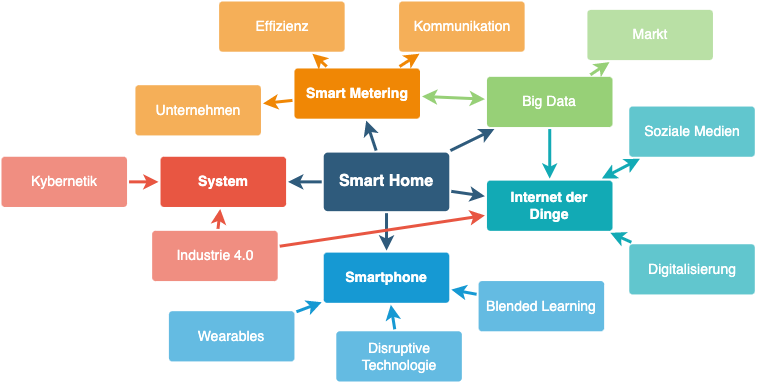
\includegraphics[width=13cm,height=13cm,keepaspectratio]{images/SH-Mind_Map.png}
            \caption{Technologische Einordnung von Smart Home in Verbindung zu IoT \cite{shmindmap2021}}
            \label{pic:mindmap_SH-IoT}
        \end{figure}
        \\
        \linebreak
        Die Abbildung (\ref{pic:mindmap_SH-IoT}) zeigt die Verbindungen als auch die Beziehungen von \acl{SH} zu anderen Technologien. Hier wird 
        deutlich, dass im Bereich des \acl{SH} viele Fragestellungen thematisiert werden können, die andere Themenbereiche tangieren.  
        \\
        \linebreak
        Um die Bezugspunkte und die Einordnung zu verstehen, wird in folgendem Abschnitt auf die Funktionsweise von \acl{SH} eingegangen.
        \\ 
        Der Aufbau eines \acl{SH} ist architektonisch ähnlich zu dem Grundprinzip einer \acs{IoT}-Lösung. Die Veranschaulichung des 
        zugrundeliegenden Aufbaus ist der Abbildung (\ref{pic:skizze_iot}) zu entnehmen. 

    \subsubsection*{Funktionsweise eines \acl{SH}}
        Ein \acl{SH} System besteht aus mehreren Teilsystemen, die in der Regel aus verschiedenen Komponenten bestehen. 
        Wichtige Elemente eines grundlegenden Aufbaus sind die Endgeräte, die sogenannten Aktoren, Eingabegeräte, 
        Sensoren, Gateway und die Vernetzung über Funk, Kabel oder Stromnetz. Die Endgeräte sind die Ausgabegeräte, die 
        über die intelligente Steuerung angesprochen werden können. Darunter zählen zum Beispiel 
        LED-Lampen, Rolläden, Lüftungsanlagen, Lautsprecher, Fernseher, Waschmaschinen und jegliche Arten von 
        Service-Robotern. Eingabegeräte sind die Schnittstelle zwischen der Interaktion des Nutzers und des 
        Smart Home Systems. Das können Wandschalter, Touchdisplays, Fernbedienungen, Smartphones und Regler sein. 
        Mithilfe dieser Schnittstelle können Zustände und Aktionen an den Endgeräten ausgelöst werden. Bei einer 
        fehlenden Verbindung zwischen den Steuerelementen sind diese trotzdem noch über direkte Schaltbefehle möglich. 
        Damit die Zustände ebenso digitalisiert werden können und dem System zur Verfügung stehen, werden Sensoren 
        benötigt. Diese greifen die physikalischen oder elektronischen Eigenschaften des Endgerätes ab, um die 
        Zustände zu ermitteln. Das Gateway repräsentiert die zentrale Steuereinheit, auf dem die Sensordaten 
        eingehen und die Sendung von Befehlen an die Aktoren stattfindet. Ebenso ermöglicht das Gateway die 
        Kommunikation der Endgeräte und Sensoren untereinander. Eine mögliche Internetverbindung zwischen 
        dem Gateway und einer zentralen Plattform, die über die Cloud erreichbar ist, kann ebenso hergestellt werden. 
        Je nach Gerät kann über das Gateway auch eine direkte Steuerung einzelner Elemente stattfinden. Das letzte 
        Element, die Vernetzung, ist dafür zuständig, die Verbindung aller Elemente. Hierfür kommen verschiedene 
        Protokolle, die unter anderem in Abschnitt (\ref{sec:technologien}) beschrieben werden, 
        per Funk, Kabel oder Stromnetz zum Einsatz. % https://www.verbraucherzentrale.de/wissen/umwelt-haushalt/wohnen/smart-home-das-intelligente-zuhause-6882#:~:text=Darunter%20fallen%20zum%20Beispiel%20Heizk%C3%B6rperregler,aus%20einem%20oder%20mehreren%20Eingabeger%C3%A4ten.
        \\
        Ein exemplarischer Aufbau der Komponenten ist der folgenden Abbildung zu entnehmen:
        \begin{figure}[hbt!]
            \centering
            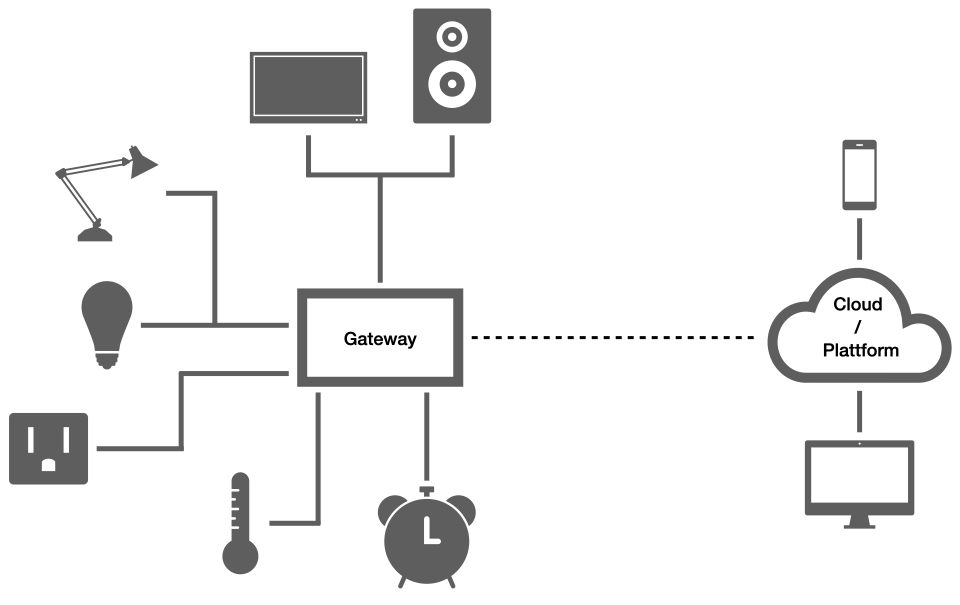
\includegraphics[width=13cm,height=13cm,keepaspectratio]{images/smart_home_connection.png}
            \caption{Aufbau und Funktionsweise einer Smart Home Infrastruktur}
            \label{pic:aufbau_SH}
        \end{figure}
        
        %Fügung in ein IoT Grundprinzip - https://www.aimprosoft.com/blog/iot-smart-home/  


    \subsubsection{Eigendefinition Smart Home}
    
    \subsection{Historische Entwicklung}
        Der Ursprung der heutigen Smart Home Bewegung ist auf die 1970er Jahre zurückzuführen. Zu dieser Zeit entstanden die ersten 
        Prototypen von Smart Home Anwendungen, die in Form von Gebäudeleitsystemen für Überwachungsaufgaben zumeist in Zweckbauten 
        umgesetzt wurden (vgl. KUSBER 2007, 11). Vorreiter war zu dieser Zeit das Unternehmen Busch-Jaeger mit dem 
        Gebäudeautomationssystem Timac X10 (vgl. ASCHENDORF 2014, 55). Rund ein Jahrzehnt später gab es eine vertiefte Forschung 
        von Bau-, Telekommunikations- und Chipherstellerunternehmen in Europa, den USA und Japan. Um eine breitere Zielgruppe 
        anzusprechen reagierten die Unternehmen mit Kooperationen und der Festlegung von Standards und Normen. Zusätzlich wurden 
        staatliche Richtlinien eingeführt. Durch diese konnte eine konsequente Förderung der vier Hauptziele Komfort, Sicherheit, 
        Ökonomie und Ökologie angestrebt werden (vgl. KUSBER 2007, 12f).
        Die erfolgreiche Umsetzung einer Kooperation eines Gebäudeautomatisierungssystems in Europa ist KNX. Dabei kam es zu einer 
        partiellen Übernahme der europaweit anerkannten Konnex Association Richtlinien in die Europäische Norm EN50090 (vgl. KUSBER 2007, 15f).

    \subsection{Ziele von Smart Home}